\documentclass[12pt]{article}
\usepackage[margin=0.5in]{geometry}
\usepackage{etoolbox}
\newtoggle{showAnswers}
\togglefalse{showAnswers}
%\toggletrue{showAnswers}% toggle this line to show/hide answers
\iftoggle{showAnswers}{ 
    \newenvironment{answer}{\vspace{1em}\color{blue!90!black}}{}
}{%
    \usepackage{verbatim}
    \newenvironment{answer}{\vspace{0em}\expandafter\comment}{\expandafter\endcomment} 
}%
\usepackage{xcolor}
\usepackage{amsfonts}
\usepackage{mathtools}
\usepackage[singlelinecheck=false]{caption}
\renewcommand\labelitemi{}% no bullets
\usepackage{sectsty}% smaller font for \section
    \sectionfont{\fontsize{12}{15}\selectfont}
\setlength\parindent{0pt}% no indents
\usepackage[colorlinks = true,
            linkcolor = black,
            urlcolor  = blue,
            citecolor = black,
            anchorcolor = black]{hyperref}
\usepackage{tikz}
\usetikzlibrary{calc}



\title{Ask Math Anything}
\author{Daily Challenge with Po-Shen Loh}
\date{16 June 2020}

\begin{document}
\begin{minipage}{\textwidth}
\maketitle
\begin{abstract}
Professor Po-Shen Loh solves problems on his YouTube channel. A selection for practice. 

Reference:~ 
\href{https://www.youtube.com/channel/UCf78EJOm4wQ4xXwSS15PuxQ}{Ask Math Anything - Daily Challenge with Po-Shen Loh}
\end{abstract}
\end{minipage}

\section*{2020/06/19}
\section{The Golden Rectangle and Golden Ratio}
The golden rectangle has the property that if you cut a square inside of it, the remaining rectangle is ``similar'' to the original rectangle, that is 
\begin{align*}
\text{The ratio}~~~ \frac{\text{length}}{\text{width}} ~~~\text{are equal}
\end{align*}
If $x$ denotes the length of the rectangle (to be determined), the proportions of the orignial and inscribed rectangles must satifsy:
\begin{align*}
\frac{x}{1} = \frac{1}{x-1}
\end{align*}
The Golden rectangle is:
\begin{center}
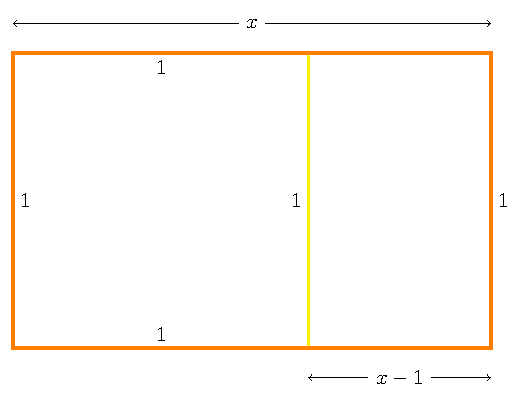
\includegraphics{tikz-rectangle-golden}
\end{center}
Rearranging the equation yields a quadratic equation,
\begin{align*}
x^2 - x - 1 = 0
\end{align*}
This quadratic equation has two real solutions, one positive, one negative (both irrational):
\begin{align*}
(x-\phi) (x-\psi) = 0
\end{align*}
where $\phi$ (pronounced `phi') is the famous golden ratio -- sometimes called the golden section:
\begin{align*}
\phi = \frac{1+\sqrt{5}}{2} \approx 1.618034
\end{align*}
and $\psi$ is the not-at-all famous negative solution of the quadratic equation:
\begin{align*}
\psi = \frac{1-\sqrt{5}}{2} \approx -0.618034
\end{align*}
Note that the repeating decimals are the same. If you cannot see why, look up Professor Po-Shen Loh's video on the quadratic equation. The golden ratio is sometimes denoted $\varphi$ (also pronounced `phi'). 

\section{The Silver Rectangle and Silver Ratio}
The golden rectangle has the property that if you cut two squares inside of it, the remaining rectangle is ``similar'' to the original rectangle, that is 
\begin{align*}
\text{The ratio}~~~ \frac{\text{length}}{\text{width}} ~~~\text{are equal}
\end{align*}
If $x$ denotes the length of the rectangle (to be determined), the proportions of the orignial and inscribed rectangles must satifsy:
\begin{align*}
\frac{x}{1} = \frac{1}{x-2}
\end{align*}
The Silver rectangle is:
\begin{center}
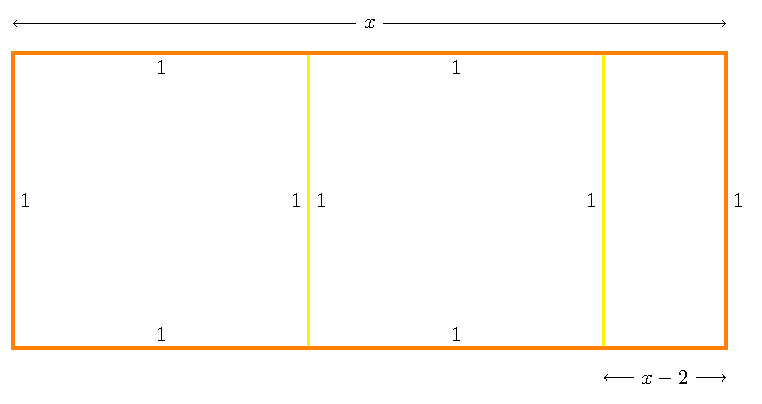
\includegraphics{tikz-rectangle-silver}
\end{center}
Rearranging the equation yields a quadratic equation,
\begin{align*}
x^2 - 2x - 1 = 0
\end{align*}
This quadratic equation has two real solutions, one positive, one negative (both irrational). The silver ratio -- sometimes called the silver mean -- is:
\begin{align*}
\delta = 1+\sqrt{2} \approx 2.414214
\end{align*}

Beware of the signs: The silver quadratic equation almost looks like $x^{2}-2x+1=(x-1)^2$. 


\end{document}